\chapter{Results and Discussion}
The starting point of this project was the familiar interdigitated qubit (see figure \ref{fig:}). This chapter will start with a discussion of the results gathered on this design.

%%The main focus during this project rested on two distinct qubit designs, namely the interdigitated and the parallel pad qubits. The two designs can be compared in figure \ref{fig:}.


First, the influence of different parameters on the capacitance of structures was determined. This knowledge enables designing structures with a specific capacitance necessary for a qubit with a certain frequency (see equation \eqref{eq:}).


Secondly, the participation ratio of the lossy layers is determined. This will give insight into what design decisions can be made to reduce these participation ratios.\\
Taking these insights into account a second qubit design was investigated in similar fashion. 





\section{Interdigitated qubit}
\subsection{The capacitance} \todo{rethink subsection structure?}
\subsubsection{Ground plane separation}
To better determine the influence of the pad design on the capacitance of the system, the influence of the ground plane is determined as a function of separation distance. Figure \ref{fig:capacitance_vs_slotsize} indicates that the influence of the ground plane on the capacitance of the system decreases rapidly with increasing separation distance. The influence of the ground plane becomes insignificant only at a separation distance of around 100 \(\mu\)m. So, in order to determine the influence of changes in pad design on the capacitance (and participation ratio) of the system, the separation distance of the ground plane should be carefully kept equal among pad designs. \todo{Or I should have eliminated the ground plane altogether when determining the influence of certain parameters.} 

\subsubsection{The fingers}
For the interdigitated pad design, the first parameter under investigation is the amount of 'fingers' in the  qubit. The capacitances of qubits with 4 to 9 fingers were determined. The finger length, width and separation were not changed.
As can be seen in figure \ref{fig:}, the relationship appears to be linear. This can be explained by viewing the addition of a finger as the addition of an extra capacitor in parallel.\\
Next the influence of the finger width is determined. The finger separation is kept equal to the finger width. For a design with five fingers the results are depicted in figure \ref{fig:} \\

Having determined the dependencies, qubits can be designed to have specific capacitances. Keeping all other parameters equal, the capacitance of earlier systems was tuned by adjusting the length of the fingers. For qubits with 5 fingers and a finger width of 5 to 50 \(\mu\)m the finger length was adjusted between 10 and 100 \(\mu\)m. \\
The results are combined in figure \ref{fig:Capacitances_g5_50}.

 

\begin{figure}
	\centering
	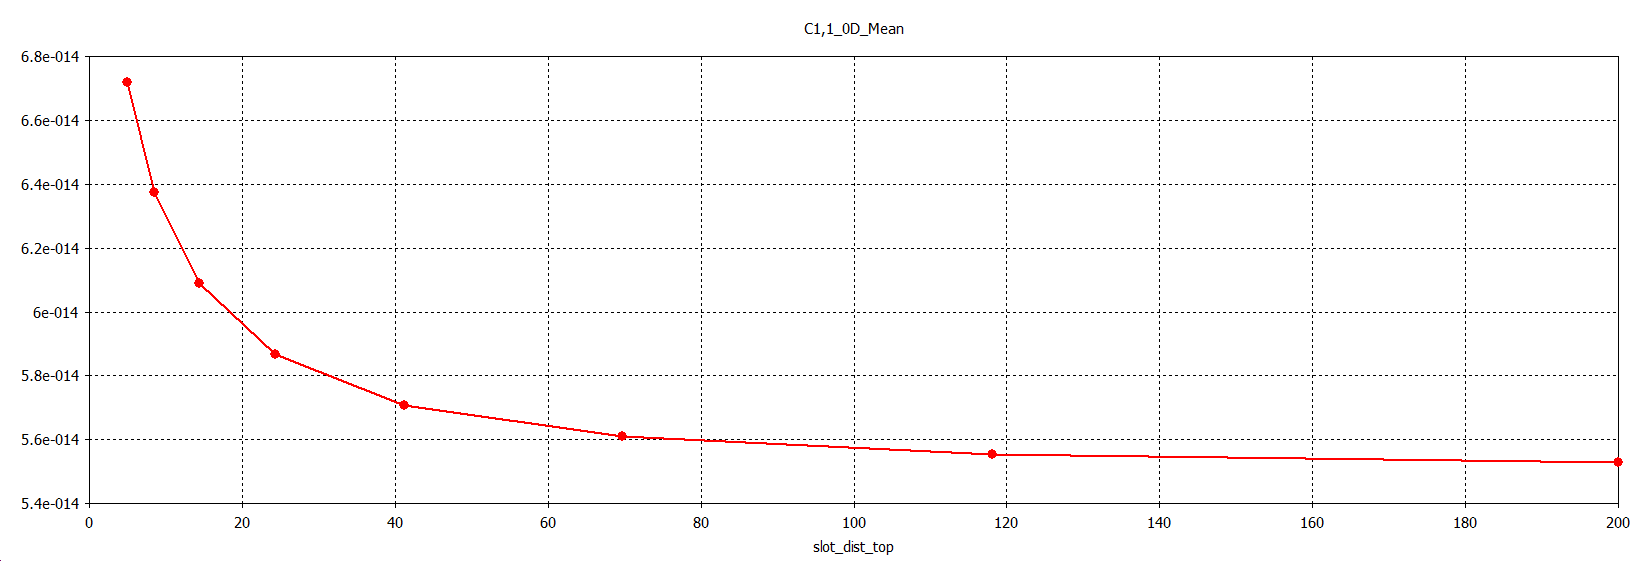
\includegraphics[width = \textwidth]{Figures/capacitance_vs_slotsize}
	\caption{Capacitance of the system as a function of ground plane separation}
	\label{fig:capacitance_vs_slotsize}
\end{figure}

\begin{figure}
	\centering
	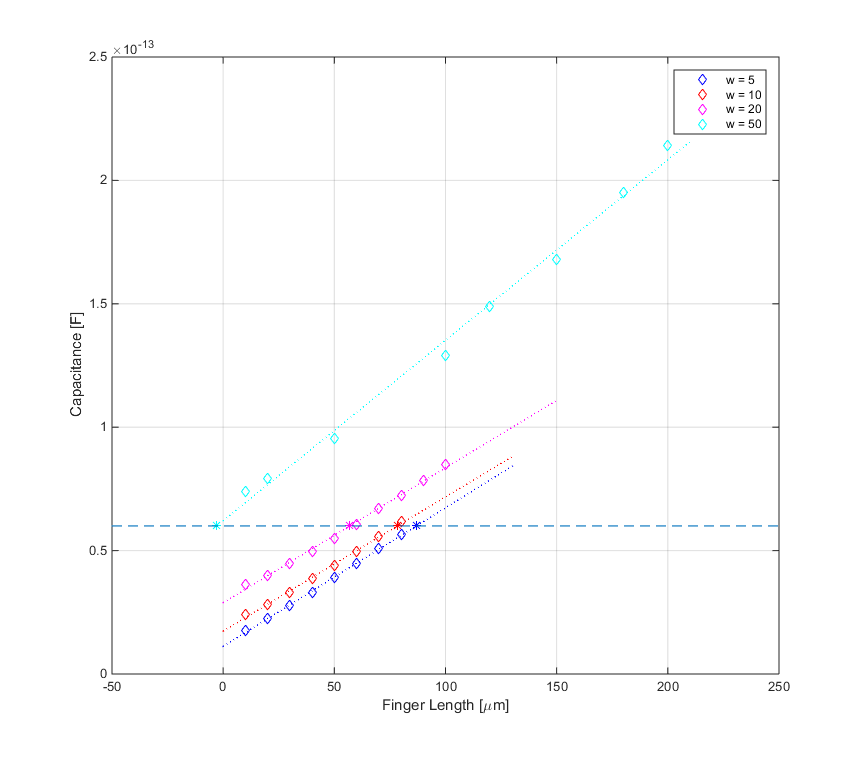
\includegraphics[width = \textwidth]{Figures/Capacitances_g5_50}
	\caption{A plot of the capacitance as a function of finger length for several finger widths. dotted lines represent linear fits of the data. The horizontal dashed line is a guideline for the eye showing the necessary finger length to make a 60\(f\)F capacitor.}
	\label{fig:Capacitances_g5_50}
\end{figure}

\section{The participation ratio}
Using the previous results several interdigitated qubits were designed to have a capacitance of 60 \(f\)F. An overview of the relevant parameters can be seen in table \ref{table:60fF_fingerlength}. The resulting participation ratios of the different lossy layers can be seen in the same table. As the finger width is increased and the finger length decreased, all participation ratios decrease. 

\begin{table}
	\begin{center}
		\begin{tabular}{ | l || c | c || c | c | c | c |}
			\hline
			Fingers  & Finger Width [\(\mu\)m] & Finger Length [\(\mu\)m]  & P ma &  Pms & P sa & P all \\ \hline
			5 & 5 & 87 & 1.85e-04 & 1.60e-03 & 4.94e-04 & 2.28e-03 \\  
			5 & 10 & 76 & 8.62e-05 & 8.45e-04 & 2.66e-04 & 1.20e-03 \\
			5 & 20 & 56 & 1 & 1 &1  & 1 \\
			10 & 5 & 36 & 1.36e-04 & 1.30e-03 & 4.12e-04 & 1.85e-03 \\
			10 & 10 & 26 & 7.56e-05 & 7.33e-04 & 2.46e-04 & 1.06e-03 \\
			\hline
		\end{tabular}
	\end{center}
	\caption{The relevant parameters for interdigitated qubit. For all designs the finger length has been tuned to result in a qubit with a capacitance of 60 \(f\)F. }
	\label{table:60fF_fingerlength}
\end{table}



By default the corners of the fingers were rounded (as in figure \ref{fig:}). As this was not standard practice the influence of doing so was determined retroactively. To do so the corner radius of the fingers (with a width of 20 \(\mu\)m) was changed between 1 and 10 \(\mu\)m (10 \(\mu\)m making semi-circles at the finger tips). The resulting participation ratios can be seen in table \ref{table:ratio_cornerradius} and figure \ref{fig:}. All participation ratios tend to decrease as the corner radius is increased. 

\begin{table}
	\begin{center}
		\begin{tabular}{ | l || c | c | c | c | c |}
			\hline
			Corner radius [\(\mu\)m] & P ma & P ms & P sa & P all \\ \hline
			1 & 1 & 1 & 1 & 1 \\
			2 & 6.57e-05 & 6.00e-04 & 1.82e-04 & 8.47e-04 \\
			5 & 6.62e-05 & 5.76e-04 & 1.78e-04 & 8.20e-04\\
			8 & 5.07e-05 & 5.25e-04 & 1.63e-04 & 7.39e-04\\
			10 & 1 & 1 & 1 & 1\\
			\hline
		\end{tabular}
	\end{center}
	\caption{caption here}
	\label{table:ratio_cornerradius}
\end{table}

The influence of the ground plane separation distance on the participation ratios was also determined. The distance was changed between 10 \(\mu\)m and 200 \(\mu\)m. The resulting participation ratios can be found in table \ref{table:ratio_groundseparation}. Again, all participation ratios show a downward trend with increasing separation distance. 

\begin{table}
	\begin{center}
		\begin{tabular}{ | l || c | c | c | c | c |}
			\hline
			Ground Separation [\(\mu\)m] & P ma & P ms & P sa & P all \\ \hline
			10 & 5.71e-05 & 5.31e-04 & 1.78e-04 & 7.67e-04 \\
			20 & 1 & 1 & 1 & 1 \\
			50 & 5.22e-05 & 5.04e-04 & 1.61e-04 & 7.17e-04 \\
			100 & 4.82e-05 & 4.92e-04 & 1.54e-04 & 6.94e-04 \\
			200 & 5.10e-05 & 4.90e-04 & 1.59e-04 & 7.00e-04\\
			\hline
		\end{tabular}
	\end{center}
	\caption{caption here}
	\label{table:ratio_groundseparation}
\end{table}

Looking at these results for the interdigitated qubit design it can be seen that the most significant change in participation ratios was achieved by making the fingers shorter and separating them further. Extrapolating these changes would indicate that a qubit consisting of two parallel rectangular pads would have even smaller participation ratios.

% \textit{Alternatively:}Extrapolating these changes would indicate that making the fingers ever shorter but wider would result in a qubit with even smaller participation ratios. The resulting qubit consists of two rectangular pads separated by the junction. 

\subsection{Parallel pad qubit}
Due to the simplicity of the parallel pad design (see figure \ref{fig:}) there are fewer ways of changing the qubit. The influence of the pad separation and the pad width on the participation ratios of the layers were determined. Comparing the the two qubit designs, increasing the finger width (and separation) in the interdigitated qubit can be seen as increasing the pad separation and pad width in the parallel pad qubit.


    